% THIS IS SIGPROC-SP.TEX - VERSION 3.1
% WORKS WITH V3.2SP OF ACM_PROC_ARTICLE-SP.CLS
% APRIL 2009

\documentclass{acm_proc_article-sp}

\begin{document}

\title{ Expresso: Typesetting Handwritten Mathematical Expressions on the Post-PC Tablet Computer }
\subtitle{ [Project Final Report] }

\numberofauthors{2} 

\author{
\alignauthor
Josef Lange\\
       \affaddr{University of Puget Sound}\\
       \affaddr{1130 NW 54th St \#617S}\\
       \affaddr{Seattle, WA 98107}\\
       \email{josef.d.lange@me.com}
\alignauthor       
Daniel Guilak\\
       \affaddr{University of Puget Sound}\\
       \affaddr{3396 Wheelock Student Center}\\
       \affaddr{Tacoma, WA 98416-3396}\\
       \email{daniel.guilak@gmail.com}
}
       
\date{16 May, 2013}

\maketitle

\begin{abstract}
This paper describes a system, Expresso, that facilitates the handwritten entry and subsequent conversion of mathematical expressionsto representational language (such as \LaTeX{}) ; completed as part of our capstone project.

Subjects approached in our project include image processing, artificial intelligence, application development for the Apple iOS platform (particularly in the tablet form factor), server development, as well as the adherence to a highly disciplined development cycle. We will attempt to most accurately and most briefly explain any uncommon concepts described hereafter.
\end{abstract}

\section{Introduction}
Throughout their history, touch devices have attempted to attain status as a ``universal tool'' -- something able to function seamlessly in their users' lives. Most humans worldwide are very familiar with handwriting, and devices from Apple Newtons, to Palm Pilots, to Pocket PCs, and now to the likes of the Apple iPad, Amazon Kindle Fire, and Microsoft Surface have tried to integrate handwriting recognition with little success since, as a result of the early adoption of keyboards as the primary input method for computers, software keyboards are more familiar and efficient in the computing context to most users.

The utility of the touch-based computer interaction has only been recently fully realized, with the nascence of the ``Post-PC'' tablet and the shift from the familiar desktop-keyboard-mouse interaction paradigm to one concerned with more direct interaction with the content on-screen. The modern tablet focuses on media consumption and so-called ``basic'' computing. In today's reality, most ``Post-PC'' tablets are powerful both in hardware and in software, supporting complex and challenging computations including the decoding of video, image processing, interpretation of multiple inputs, managing several network connections, and displaying high-resolution two- and three-dimensional graphics. In addition, and perhaps in part as a result, to their technical prowess, ``Post-PC'' tablets have developed a near-ubiquity in the computing world.

For the usage described, the touch interface of a ``Post-PC'' tablet offers a unique tool---the direct input of figures via touch---that has only previously been common to those willing to purchase accessories generally intended for graphics and imaging.

Expresso sets out to take advantage of this new ubiquity in direct-interaction computing by positioning itself as an alternate input method for document production. Expresso is an application (and system of support applications) for the ``Post-PC'' tablet utilized for converting drawn mathematics into \LaTeX{} code. A user with a tablet device can open Expresso, write out an expression (valid or not) and have Expresso identify and convert the mathematics into \LaTeX{}, easily insertable in a document on which he or she is working.

\section{Related Work}
Handwriting recognition is a complex problem, only a segment of which our system wishes to solve. Existing solutions to handwriting recognition exist, and some perform at a useable level. One such example is VisionObjects MyScript\footnote{http://www.visionobjects.com/en/myscript/about-myscript/}, a commercial product that has seen significant success. Most systems require a period of ``training'' before any recognition can be achieved, relying on Artificial Intelligence concepts to deduce the symbols related to drawn squiggles on-screen. Commercial products exist, including but not limited to software built into Microsoft's Windows and Apple's Mac OS X Operating Systems. Additionally, third-party companies have produced software for a similar purpose, such as the aforementioned MyScript. Academic projects, including those by Matsakis\cite{matsakis_recognition_1999}, Smithies et. al.\cite{smithies_handwriting-based_1999}, and Levin\cite{levin_cellwriter:_2007} exhibit valid solutions for the desktop model of usage, though are not implemented in a way that is ultimately accessible for the modern possibility of the ``Post-PC'' tablet as an input method, requiring the user to have an graphics tablet which is only useful for a small set of tasks. 

Levin's project, CellWriter, was of particular interest to us, as it was also the work of an undergraduate computer science student. This made our goal seem slightly more realistic, at least to us. CellWriter, however, had some limitations which we had hoped to avoid. One, the software depended on the user writing each symbol in a predetermined cell, an option that simply is not realistic in our application. Further, this project expects each instance of the software to have one sole user, so that it can learn the way \emph{that} user specifically writes. Again, we wanted a solution more capable in terms of being useable by multiple users.

\section{Proposed Solution}
This project's goal was to produce a feature-complete, usable piece of software for the Apple iOS platform, supported by a ``cloud-based'' application. This software would have a singular function: to capture handwritten mathematical expressions via the digitizing screen, and communicate with the cloud application and compile the interpreted characters into the appropriate mathematical representational language (namely \LaTeX{} or MathML).

To use the software successfully, a user would first open the Expresso application on their iPad or iPhone. From there one would follow the on-screen instructions to ``connect'' to the cloud system. Once the connection has been established successfully, the user is invited to draw their mathematics on-screen, with options to change stroke width, undo, redo, or clear their drawing. From there, the user can select to send the image for processing, whereupon the application transmits the image along with identificating metadata to the could system. The cloud system then processes the image, selecting individual contours in the image and associating a ``best-guess'' symbol with the drawing. The cloud system then transmits back the ``guesses'' to the client application, which displays the ``guesses'' to the user. The user then has an opportunity to correct any mistakes the cloud system has made, and can then issue the command to compile the mathematics into useful code. From there, the cloud system would analyze the relative location and size of the various symbols to extrapolate the mathematical representation of the symbols, compile said representation into \LaTeX{} code, and return it to the client application, which would display the code, a rendering, and options to transfer the code to the clipboard or an email. This process is outlined (in a more simple manner) in Figure~\ref{fig:user_workflow}.

\section{Motivation \& Importance}
Both authors at one point or another have been frustrated with a homework assignments requiring mathematical typesetting in \LaTeX{}.  We believe it would be great for a user to jot down an equation on an iPad or other tablet device and have the \LaTeX{}\ code appear on the document they are editing on their laptop or desktop computer.

This software could easily improve the classroom environment in all levels of schooling. Getting mathematical equations into type is a frustrating task for many teachers in the K-12 levels, and even frustrating for the higher-education professor and student. With this software, student and educators alike can easily convert their glyphic mathematical thoughts into usable typesetting language. This will hopefully open doors to clearer and more specific teaching and learning throughout all levels of education.

\section{Method \& Implementation}

\subsection{Overview}
A large-scale application such as Expresso requires the use of a myriad of different technologies which must all work together in harmony --
the entirety of which is colloquially called ``The Stack.'' As the authors are financially unstable university students, it was necessary to
assemble a stack with little to no monetary obligation. Such a task is commonly called ``bootstrapping'' -- a reference to the idiom ``to pull one up by one's bootstraps,'' which we will often cite as reasons we opted to use open-source libraries and free services despite the fact that their premium equivalents generally are better documented and occasionally less buggy. The authors are also happy to release Expresso and its related applications under an open-source license as a serendipitous side-effect of the bootstrapping process.

The software components of this project stand upon a foundation of three central parts, as generally depicted in Figure~\ref{fig:final_chart}. The primary and most visible component is the client application, Expresso, with which the user directly interacts. Expresso communicates with Barista, the ``front-end'' server hosted on Heroku, via a RESTful API which communicates with ``Bean'' and its related applications, the server which performs all of the computationally intensive work -- image manipulation and symbol recognition -- hosted on Amazon EC2.

\subsection{``Expresso'' (iOS Client)}
The iOS client for Expresso is the face of its distributed computation system. The user directly interacts with Expresso on his or her iPad, iPhone, or iPod touch, and is able to interact with each step of the recognition and identification process. The application itself was developed using Apple's Xcode IDE, freely available to any developer with access to Apple hardware and an up-to-date version of Mac OS X.

The programming language most commonly used when developing iOS applications is Objective-C, a superset of ANSI C that gives a solid syntax for object-oriented programming. This syntax is a little bizarre at first glance, but is really powerful for rapid development of easily-readable code, in the way that the syntax will commonly read left-to-right and with non-cryptic, fully-expanded object, method, and variable names which combine to make code in Objective-C read a lot like English.

The availability of first-party frameworks from Apple for developer use is plentiful; if you need to do something you think is more than trivial, chances are there is a class and/or method for that already written. For example, if a developer needs to present a new view controller in a modal manner, the \texttt{UIViewController} class has a method called \texttt{presentModalViewController:animated:} which does just that (and allows the developer to declare whether or not said presentation should be animated). This is obviously just one example, but upon exploring the Apple's documentation of these frameworks, one will observe the existence of classes and methods to fill many intuitive needs.

iOS development is build upon the foundation of the Model-View-Controller software architecture pattern. Each class should fall into one of these three categories, and there are ``rules of thumb'' as to how members of each category interact. A model class encapsulates data utilized by applications. A view is a means by which we see data, whether it is an image view, a table view, a text view, or something like a button. What remains, then, is the controller, the real hard worker of the three categories. A controller is responsible for, to some degree, ``running the show''. Controllers interact with model objects to see and manipulate data. Controllers, too, interact with view objects in order to either change what the view is showing or doing, or to receive information pertaining to user interaction.

\begin{figure*}
\centering
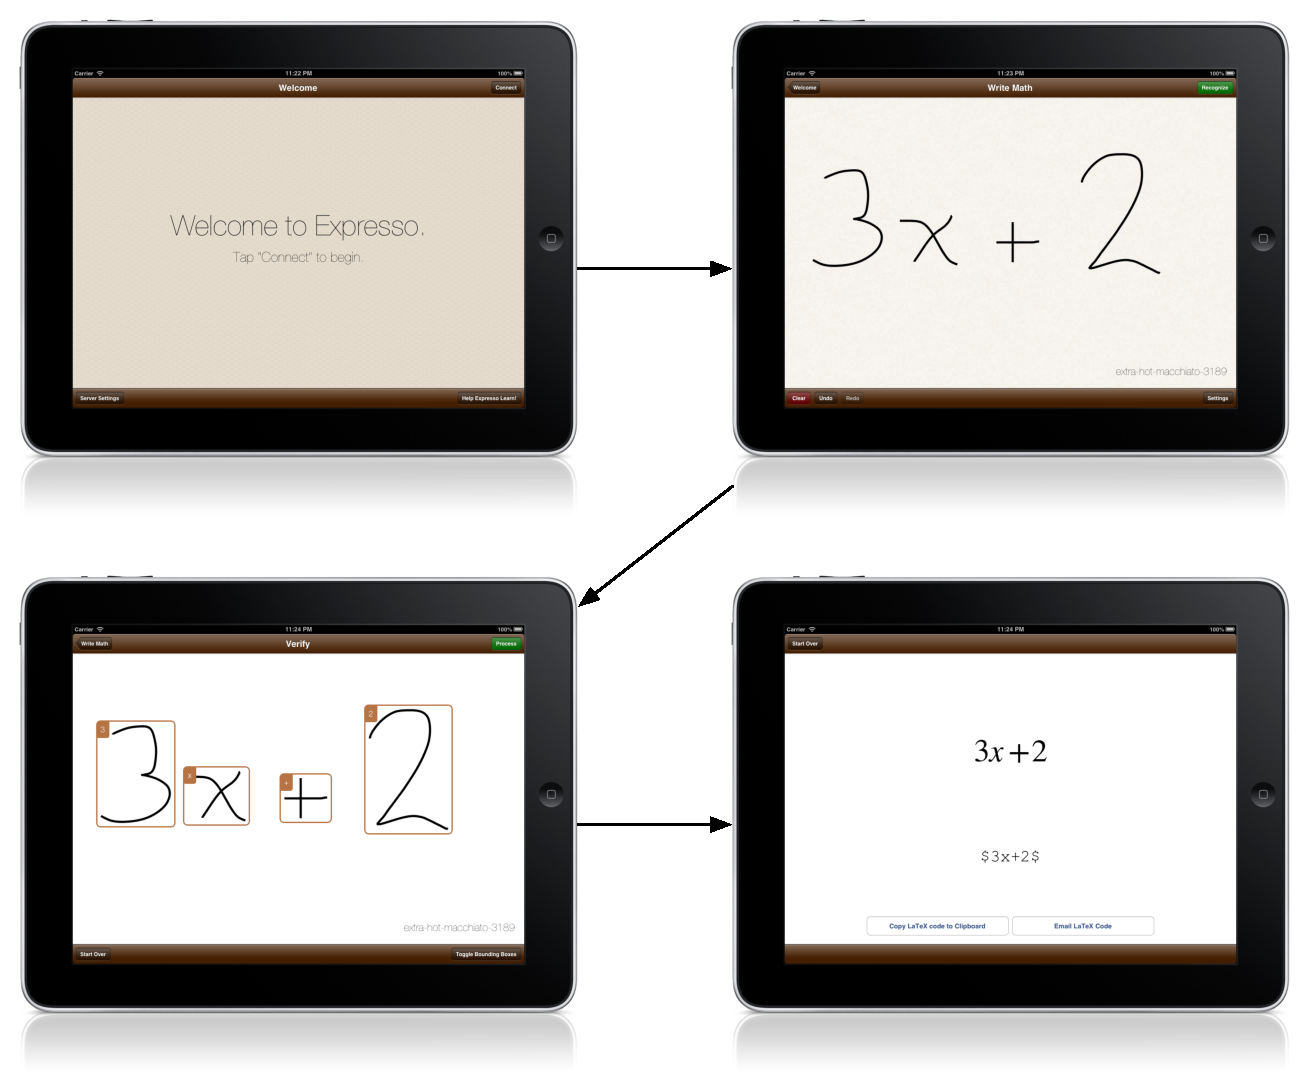
\includegraphics[width=1.0\textwidth]{user_workflow.pdf}
\caption{General User Interaction with Expresso. The user first connects to the web application. Then, they draw their math and send it off. The server returns to the client the recognized symbols. At this point, the user has the opportunity to correct any mistakes Barista and Roaster may have made. Finally, the user requests the crunched-out math and \LaTeX{} code.}
\label{fig:user_workflow}
\end{figure*}

One of the more challenging elements of the iOS client app was the drawing section. Unfortunately, there is no built-in Apple-developed framework for the capture of drawings on-screen. There does exist, however, the ability to detect and track a continuing touch and drag across the screen. Since the device cannot simply record every point touched down to an infinitessimal scale, iOS instead records position data at 60Hz.

To simply draw a line segment ``connecting the dots'' was not very good-looking. By responding to this event appropriately, we were able to implement a curve-approximating algorithm based on a tutorial found online at ``MobileTuts+''\footnote{http://mobile.tutsplus.com/tutorials/iphone/ios-sdk\_freehand-drawing/}. The algorithm remembers each point in the touch/drag in sequence and in doing so approximates a bezier curve given the point's values. This approximation's mathematics is handlede by the Apple-provided \texttt{UIBezierPath} class, which provides a method to create a curve from a point to a given point using two given control points to influence the magnitude and direction of the curve. The algorithm also re-places each point between each series of four to an average of the tail and head of the previous and next curve respectively. Each curve is its own object containing vector data (rather than bitmap of the rendered curve). As more curves are drawn on-screen, the performance can be significantly affected as the system needs to render and re-draw the paths on each refresh. The solution to this is to cache a rendered bitmap of all the previous curves, rendered, each step along the way. 

This algorithm had some drawbacks which we had to work around. First, the user would not be easily able to draw a single point. Instead, they would have to draw a small circle on-screen, which is not ideal. A special case was added to the code to accomodate a curve within a certain threshold of size to be drawn as a filled circle of that size on-screen, instead of whatever input the user actually put in. Further, the method of maintaining only one cached image and not retaining the path objects of previously-drawn paths more or less ruled out the possibility of maintaining an undo/redo stack. To get around this, previously-drawn paths were not thrown out but instead retained in a Model object, \texttt{EXDrawing}, and used to reconstruct a rendered version of a previous or future state of the drawing.

In addition to the code adapted from the tutorial on ``MobileTuts+'', the iOS client utilized two open-source projects: \texttt{ASIHTTPRequest}\footnote{http://allseeing-i.com/ASIHTTPRequest/} (BSD License) and \texttt{MBProgressHUD}\footnote{https://github.com/jdg/MBProgressHUD} (MIT License). \texttt{ASIHTTPRequest} is a collection of classes making \texttt{HTTP} requests rather straightforward and convenient to implement in code, a necessity for this project. \texttt{MBProgressHUD} was a nice compilation of views which made displaying modal progress displays (whether determinate or indeterminate) more streamlined.

The Xcode project for Expresso comes in at just under five thousand lines of code, separated into seventeen different classes. It compiles and runs on iOS devices running iOS 5 or above, though iPads running iOS 6 are the optimal target.

\subsection{``Barista''}

\begin{figure*}
\centering
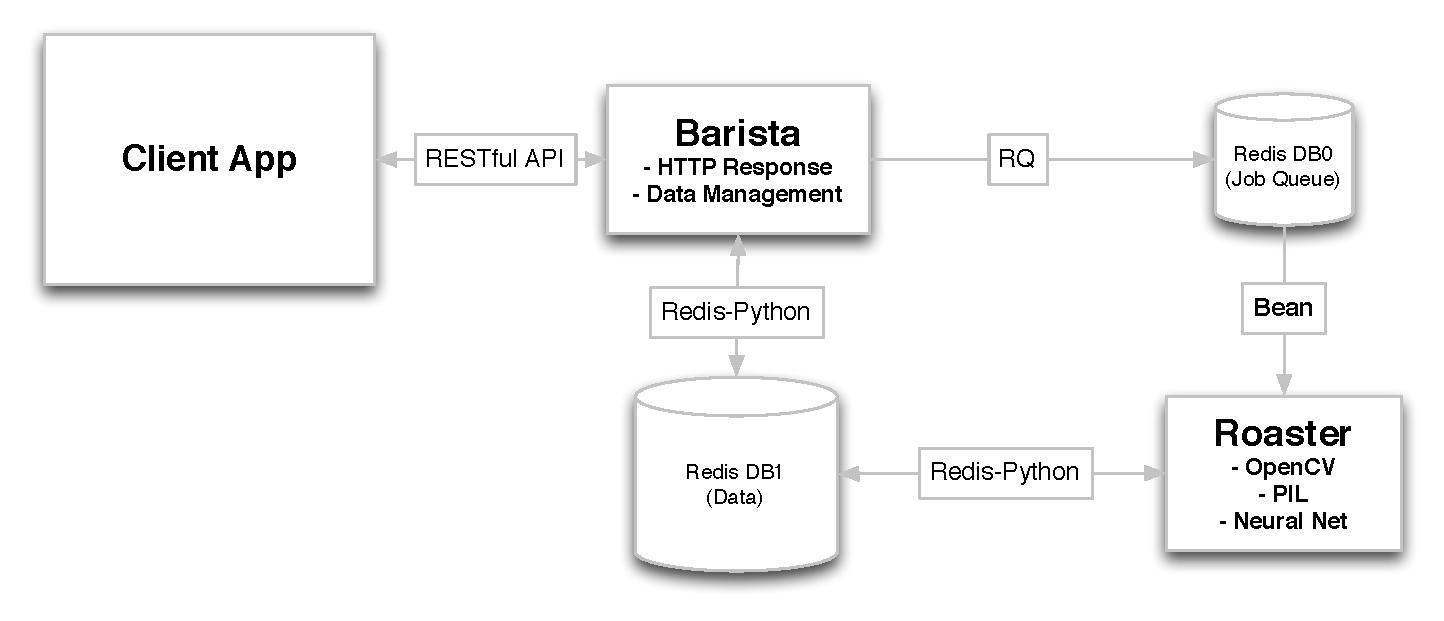
\includegraphics[width=1.0\textwidth]{final_chart.pdf}
\caption{Simplified Organization of Software Components}
\label{fig:final_chart}
\end{figure*}

A barista, in a coffee shop, is the person who takes one's coffee order and completes and delivers one's drink. Likewise, Expresso's Barista takes requests for information and delivers said information. The most fitting method of data transmission for our use was that of a RESTful API. REST, or Representational State Transfer, ``is a coordinated set of architectural constraints that attempts to minimize latency and network communication, while at the same time maximizing the independence and scalability of component implementations.''\cite{Fielding:2002:PDM:514183.514185}. In essence, REST relies on the fact that no two entities are ever automatically in-sync with one another; an entity can request data from another and manipulate it, but it must send the updated data back to its source to keep changes consistent across a system. REST has, as of late, become a \emph{de facto} standard amongst software developers looking for a server-client architecture. 

REST is but an idea; there is no official standard to adhere to, nor a strict set of guidelines upon which to build one's API. Fortunately, there exist already-implemented frameworks for the rapid development of REST-minded API server. One such tool is Flask-RESTful\footnote{https://github.com/twilio/flask-restful}, a BSD-licensed Python library that creates a framework for constructing a RESTful API on top of a web server operated by Flask\footnote{http://flask.pocoo.org}. Flask itself is an extremely lightweight web server, also available under the BSD license.

Barista leverages these technologies to serve and receive the data Expresso needs. Of course, every web application software requires web server hardware. For Barista, we selected Heroku\footnote{http://heroku.com}, a simple deployment platform for web application software, particularly those programmed in Python or Ruby (we used Python). Launching an application on Heroku requires just signing up for an account and using Git source control\footnote{http://git-scm.com} to push your code to your account on their servers. Heroku remains free to developers so long as they only run one process at a time. This, of course, presented issues when we wanted to keep our system components modular, particularly when it looked as though the recognition would need to be running a process of its own. The discussion in Subsection \ref{subsection:roaster} explains our workaround to such an issue.

Barista, since it is a web server, communicates using the \texttt{HTTP} Protocol. In particular, Barista utilizes the \texttt{GET} and \texttt{POST} methods of the \texttt{HTTP} Protocol specification. Their function is rather straighforward; \texttt{GET} requests and expects to receive data, while \texttt{POST} sends and expects the remote updating of data. 

Having an API defined convenient, but what about the data itself? \texttt{JSON}\footnote{http://www.json.org} proved most convenient for data representation in our case. \texttt{JSON} is a commonly-used standardized data format. It supports singular generically-typed elements, and the basic collections of arrays and dictionaries. Utilizing a common vocabulary of keys for requesting values, several different platforms can utilized \texttt{JSON} data without requiring any transformation of the data. Where, then, is the data stored? We ended up utilizing the Redis\footnote{http://redis.io/} NoSQL database system (again BSD-licensed), essentially a very large map of key-value pairs. This allowed us to define our own relationships in code and define and manipulate structures of data on-the-fly. To access Redis, we utilized the Python interface to Redis, redis-py\footnote{https://github.com/andymccurdy/redis-py} (under MIT license).

So, with all this in mind, we designed and developed a two-piece system for Barista. The front-side was essentially a fa\c{c}ade design pattern. It hooked into Flask-RESTful to implement the methods called when certain \texttt{HTTP} requests were made to the server at certain URL paths. Each of these methods utilized the Barista's back-side, a series of classes to Pythonically encapsulate the data stored in the Redis database for our use. Each class has the ability to detect whether or not it is ``dirty'', that is, whether or not the data the object contains is at the same state as its original data in the Redis database. This allows us to instantiate an object from the Barista module, load data into it, manipulate it, and then put the data back. It's almost a RESTful methodology in and of itself.

\subsection{Server Back-end}
Three components of Expresso -- Bean, Roaster, and Grinder -- are grouped together because they comprise the so-called ``powerhouse'' of the application as they perform all of the computationally-intensive work: image manipulation and symbol recognition. We decided to host these components separately on an Amazon EC2\footnote{http://aws.amazon.com/ec2/} virtual server T1-micro instance rather than as  additional processes on the Heroku instance which proved to be financially prohibitive, while Amazon EC2 is free for the first year. 

\subsubsection{``Bean'' (Task delegation)}
As there is a lot of work for the back-end to complete, it was in our best interest to
implement a system that would allow us to take advantage of all of the virtualized server's resources. Towards that end, we decided on using RQ\footnote{http://python-rq.org/}, a Python library for implementing a priority task queue in a Redis data-structure server instance residing on our server. Barista (on Heroku) submits various different jobs to the RQ task queue on the EC2 instance, and Bean is the worker (technically a modified instance of `rqworker`) that monitors its status and pops tasks off to delegate to Roaster (image manipulation) and Grinder (symbol recognition).

There are many advantages to implementing this sort of architecture. The ability to vary priority levels for different tasks allows us to make sure that important and time-sensitive jobs (e.g., those that directly impact the user like symbol recognition) will receive computational attention before ones that are not necessarily imperative (e.g., adding additional data to the symbol recognition data set) for regular function. In addition, Bean allows for scalability as well. Multiple Bean instances can be running on the same machine (or even different machines!) to be able to pull and delegate jobs -- all that is required is that they be able to connect to the Redis instance, whether locally or over the Internet.

\subsubsection{``Roaster'' (Image processing)}
When the user draws an expression, it is saved in a bitmap format and transferred through Barista and to the RQ task queue where Bean delegates the task of splitting up the image into different symbols to Roaster.

In essence, Roaster is a set of methods that use the Python Imaging Library (\texttt{PIL})\footnote{http://www.pythonware.com/products/pil/}, \texttt{OpenCV}\footnote{http://opencv.org/}, and \texttt{NumPy}\footnote{http://numpy.org/} libraries to calculate bounding boxes for each symbol (the result of which can be seen in the bottom-right corner of Figure~\ref{fig:user_workflow}) and save them as separate grayscale bitmaps that could be passed on to Grinder for symbol recognition.

\label{subsection:roaster}
\subsubsection{``Grinder'' (Symbol recognition)}
We made many different attempts at developing an easy-to-understand and effective symbol recognition engine (see: \emph{Section 6}). Ultimately, we decided to use \texttt{OCRN}\footnote{https://github.com/swvist/Ocrn/}, a simple open-source handwriting recognition engine by Vipin Nair using functionality from \texttt{PyBrain}\footnote{http://pybrain.org/}, a python machine learning library.

We heavily modified \texttt{OCRN} to suit our needs. Essentially, it provides an implementation of a neural network, which is an artificial network which mimics the manner in which neurons communicate and learn information in a brain. Two integral components comprise Grinder: a neural network and a supervised data set for its training. The neural network's default parameters are 100 input nodes (one for each vector in the symbol image), 80 hidden layers, and the dimension of output equal to one (only one output ASCII value).

When in training mode, Grinder takes a number of grayscale symbols from Roaster labelled with the appropriate ASCII value and stores them in the supervised data set, and then trains the neural network on the data set until it reaches convergence. When Bean submits a request for symbol recognition, Grinder simply activates the neural network with the symbol as an argument, and the network returns the most likely ASCII value that the unknown symbol represents, which is then stored in the Redis database for easy access via Barista and the RESTful API.


\section{Evaluation}
Tackling such a large-scale implementation project part-time proved to be a challenging yet rewarding task. In that, there were aspects of the application which we believe we completed to our standards, and others that we would have liked to improve upon given more time.

\subsection{Successes}
\begin{itemize}
	\item{\emph{Financial Requirement}} -- With the bootstrapped nature of Expresso, DG and JL were able to develop this system without any sort of monetary investment in libraries or services.
	\item{\emph{Scalability}} -- By using platforms such as Heroku and Amazon EC2 for hosting and technologies like Redis and the RQ task queue system (Bean), we designed the Expresso system to be able to easily scale up, were it ever to reach a large number of users.
	\item{\emph{Portability}} -- With the implementation of RESTful techniques on Barista, it would be a trivial exercise to port the Expresso application from iOS to Android, a web application, or any other sort of device that could interface with the API.
	\item{\emph{Open Source}} -- Due the use of many different open-source libraries and applications, we are able to release our project under an open-source license on GitHub\footnote{http://github.com/expresso-math/}.

\end{itemize}

\subsection{Failures}
\begin{itemize}
	\item{\emph{Ineffective Symbol Recognition}} -- Despite having tried numerous different open-source symbol recognition systems such as \texttt{Tesseract}\footnote{https://code.google.com/p/tesseract-ocr/}, \texttt{OCRopus}\footnote{https://code.google.com/p/ocropus/}, \texttt{OpenCV}, and \texttt{OCRN}, we were still unable to implement an accurate optical character recognition system due to a lack of knowledge of Machine Learning and poor documentation.
	\item{\emph{Poor Task Triage}} -- We frequently found ourselves hung up on the fact that our symbol recognition was not functioning properly, and spent many man-hours debugging and trying various different libraries and applications, while it would have been wise of us to instead use some of that time developing the mathematical parsing system which we were unable to complete in the time allotted.
	\item{\emph{Unfinished Product}} -- Due to all of the reasons listed above, sadly we were unable to complete all of the goals we set out to accomplish.
	
	\end{itemize}

\subsection{Future Work}
Moving forward, the obvious path is to select or outrightly build a recognition engine that actually works. That might be a matter of looking harder, waiting until someone actually does it, or becoming incredibly intelligent and perceptive in the ways of the neural network. From there, we'd be able to implement expression generation, which is outlined in several academic articles.

We also have yet to design and implement the web client that would allow the realization of our original use case -- someone working on a \LaTeX{}  document and inputs a mathematical equation to insert on their iOS device, and the equivalent \LaTeX{}  code appears on a web client on their desktop or laptop machine. Completion of this task is trivial compared to the complicated AI requirements for other portions of this project.

In the very distant future, we would also like to implement a minimal social-networking aspect to the application that would allow people to share their formatted equations with each other -- which would bring some haste to the time-hungry field of academia.

\section{Discussion \& Analysis}
Throughout the process of development, we ran into several challenges, some of which we successfully worked through or around, others we did not. Among these challenges were character recognition, image processing, poorly-documented resources, and a proclivity for getting ``hung up'' on a particular issue.

Na\"{i}vely, we assumed that the smaller set of symbols to be recognized (digits and operators as opposed to letters) would make the recognition process easier. While it is true in some sense, the ease it gains is in increased accuracy of a working recognition engine. We didn't have one of those. We shuffled through several recognition engines and implementations of various forms of Artificial Intelligence, none of which seemed capable of successfully identifying symbols. This, obviously, caused a large issue that cascaded into other segments of the project. Because we yearned so desperately to have recognition work, we found ourselves essentially wasting time trying to get recognition to work instead of moving on to other components of the project.

The image processing involved in preparing an image for recognition is suspect to some of our problems. Neither of us were particularly familiar with the technique behind image encoding and still know very little. Our use of \texttt{OpenCV} and \texttt{PIL} was guided by poor documentation and, most of the time, nearly-wild guesses. Perhaps a stronger understanding of images and how one can represent them for input to a Neural Network, for example, might have served us better as we tackled the recognition problem.

The most stark of challenges was certainly symbol recognition, as mentioned above. In addition to our inability to successfully recognize symbols, we found that we simply ran out of time to begin implementation of expression generation. As such, for demonstration purposes, we constructed a ``fake'' engine that spits out the same value for every expression. Not useful in the real world, but as a means to show how the application would work, we were happy with the results.

\section{Conclusion}
Expresso was a challenging project to undertake and one that required focused work and the complete education of a computer science major. At the most basic level, it required a lot of programming, and smart programming at that. The intelligent use of basic programming skills and data structures was crucial to the success of the project. Understanding the complexity of algorithms and their efficiencies was equally important in tuning certain features to work within the bounds of acceptable timing. Image processing and the transfer of image data required an understanding of the architectual representations of data on the bit-to-bit level. Artificial intelligence was an obviously critical element to the project as well. On the higher-level, the concepts of software engineering became crucial as the software became divided into so many pieces. 

Regardless of the project's success as measured by its ability to complete the tasks intended, the process of development, its rigor, and our ability to navigate through it, we feel, is a clear display of concepts learned at the University of Puget Sound and a reflection of the high ambitions we have developed as a result.

\section{Acknowledgements}
JL and DG would like to thank Prof. Joel Ross for providing mentoring support throughout this project, and the University of Puget Sound for a quality education in Computer Science -- both theoretical and technical.

%\end{document}  % This is where a 'short' article might terminate

\bibliographystyle{abbrv}
\bibliography{final_citations}  
% You must have a proper ".bib" file
%  and remember to run:
% latex bibtex latex latex
% to resolve all references
%
% ACM needs 'a single self-contained file'!
%
%APPENDICES are optional
%\balancecolumns


\balancecolumns

% That's all folks!
\end{document}
